\documentclass[conference]{IEEEtran}
\IEEEoverridecommandlockouts
% The preceding line is only needed to identify funding in the first footnote. If that is unneeded, please comment it out.
\usepackage{cite}
\usepackage{amsmath,amssymb,amsfonts}
\usepackage{algorithmic}
\usepackage{graphicx}
\usepackage{textcomp}
\usepackage{xcolor}
\def\BibTeX{{\rm B\kern-.05em{\sc i\kern-.025em b}\kern-.08em
T\kern-.1667em\lower.7ex\hbox{E}\kern-.125emX}}
\begin{document}

\title{Accordion Autoencoder $(A^2E)$ for Improving Classification Performance}

\author{\IEEEauthorblockN{1\textsuperscript{st} Kevyn Kelso}
    \IEEEauthorblockA{\textit{Department of Electrical and Computer Engineering} \\
        \textit{University of Colorado at Colorado Springs}\\
        Colorado Springs, Colorado \\
    kkelso@uccs.edu}
    \and
    \IEEEauthorblockN{2\textsuperscript{nd} Dr. Byeong Kil Lee}
    \IEEEauthorblockA{\textit{Department of Electrical and Computer Engineering} \\
        \textit{University of Colorado at Colorado Springs}\\
        Colorado Springs, Colorado \\
blee@uccs.edu}}

\maketitle

\begin{abstract}
\end{abstract}

\begin{IEEEkeywords}
\end{IEEEkeywords}

\section{Introduction}
Autoencoder networks have applications in dimensionality reduction, input reconstruction, anomaly detection, and classification problems. As a methodology for dimensionality reduction, the lower dimensions can generalize sets of higher dimensions which yield intuitive feature responses. In modern applications, generative models have lower dimensional latent spaces which can be manipulated to change features of the output. Most recently, autoencoders have also been used in quantum data compression problems.

Autoencoders are not used in practical data compression problems because modern algorithms have better performance without the required training. It would also be impractical to gather a dataset for each compression application due to autoencoder networks having poor performance on dataset transfer learning. This lack of dataset flexibility is one of the main reasons why autoencoders are great for anomaly detection. Once the autoencoder network is trained on particular data, any data fed through the network slightly outside the training data results in a high reconstruction loss.

The motivation behind exploring different autoencoder architectures lies in their practical uses for the application such as anomaly detection (fraud dataset) and classification (MNIST dataset) and their usages in generative models where latent space is manipulated to generate novel output. Additionally, understanding different ways to improve dimensionality reduction techniques may lead to a better understanding of how the human brain finds meaning in data.

Classic implementations of autoencoders for anomaly detection have many false positives resulting in low precision and F1 scores. Sensitivity analysis-based architecture design can be used to not only reduce the false positives but also increase overall performance, but potentially increase the recall score too leading to better separation between classification and anomaly detection categories. In addition, architectural network design should target decreases in network complexity allowing more efficient implementation, faster training, and faster prediction speeds with no cost to the other metrics mentioned above.

As a better performing solution to anomaly detection and classification problems, this paper introduces a different autoencoder architecture which is not necessarily a solution to dimensionality reduction, but rather a performance improvement for these problems using several sets of lower dimensional space to encourage more meaningful generalizations of the data as a whole. Two applications of this architecture were explored; anomaly detection in credit card transaction data, and image classification using the MNIST dataset. A performance improvement in both datasets was seen using the new autoencoder architecture.

In this paper, we proposed an accordion autoencoder architecture, as a better performing solution to anomaly detection and classification problems, which is not necessarily a solution to dimensionality reduction, but rather a performance improvement for the problems using several sets of lower-dimensional space to generate more meaningful generalizations of the data as a whole. Two applications are used for our experiments; anomaly detection in credit card transaction data, and image classification using the MNIST dataset. Based on our experiments, the proposed solution provides network size reduction with maintaining accuracy.

\section{Characterization of AUTOENCODERS}
An autoencoder is a fully connected neural network meant to compress the input into a smaller and more meaningful representation, then decoding that representation into an output resembling the original input [1]. Usually, reducing the dimensionality of the input is the goal of the autoencoder. The lower-dimensional vector which is the smallest middle layer is commonly called the latent space. Ideally, the autoencoder learns distinguishable attributes of the data which are represented in the latent space. These attributes tend to be generalizations of the data representing one or many features in the input. The latent attributes can sometimes resemble the results of principal component analysis but often perform better due to the nonlinearity of the encoder and decoder layers [2]. Figure 1 shows a 5 layer autoencoder with 2 layers of encoding, 1 layer of latent space, and 2 layers of decoding.

\begin{figure}
    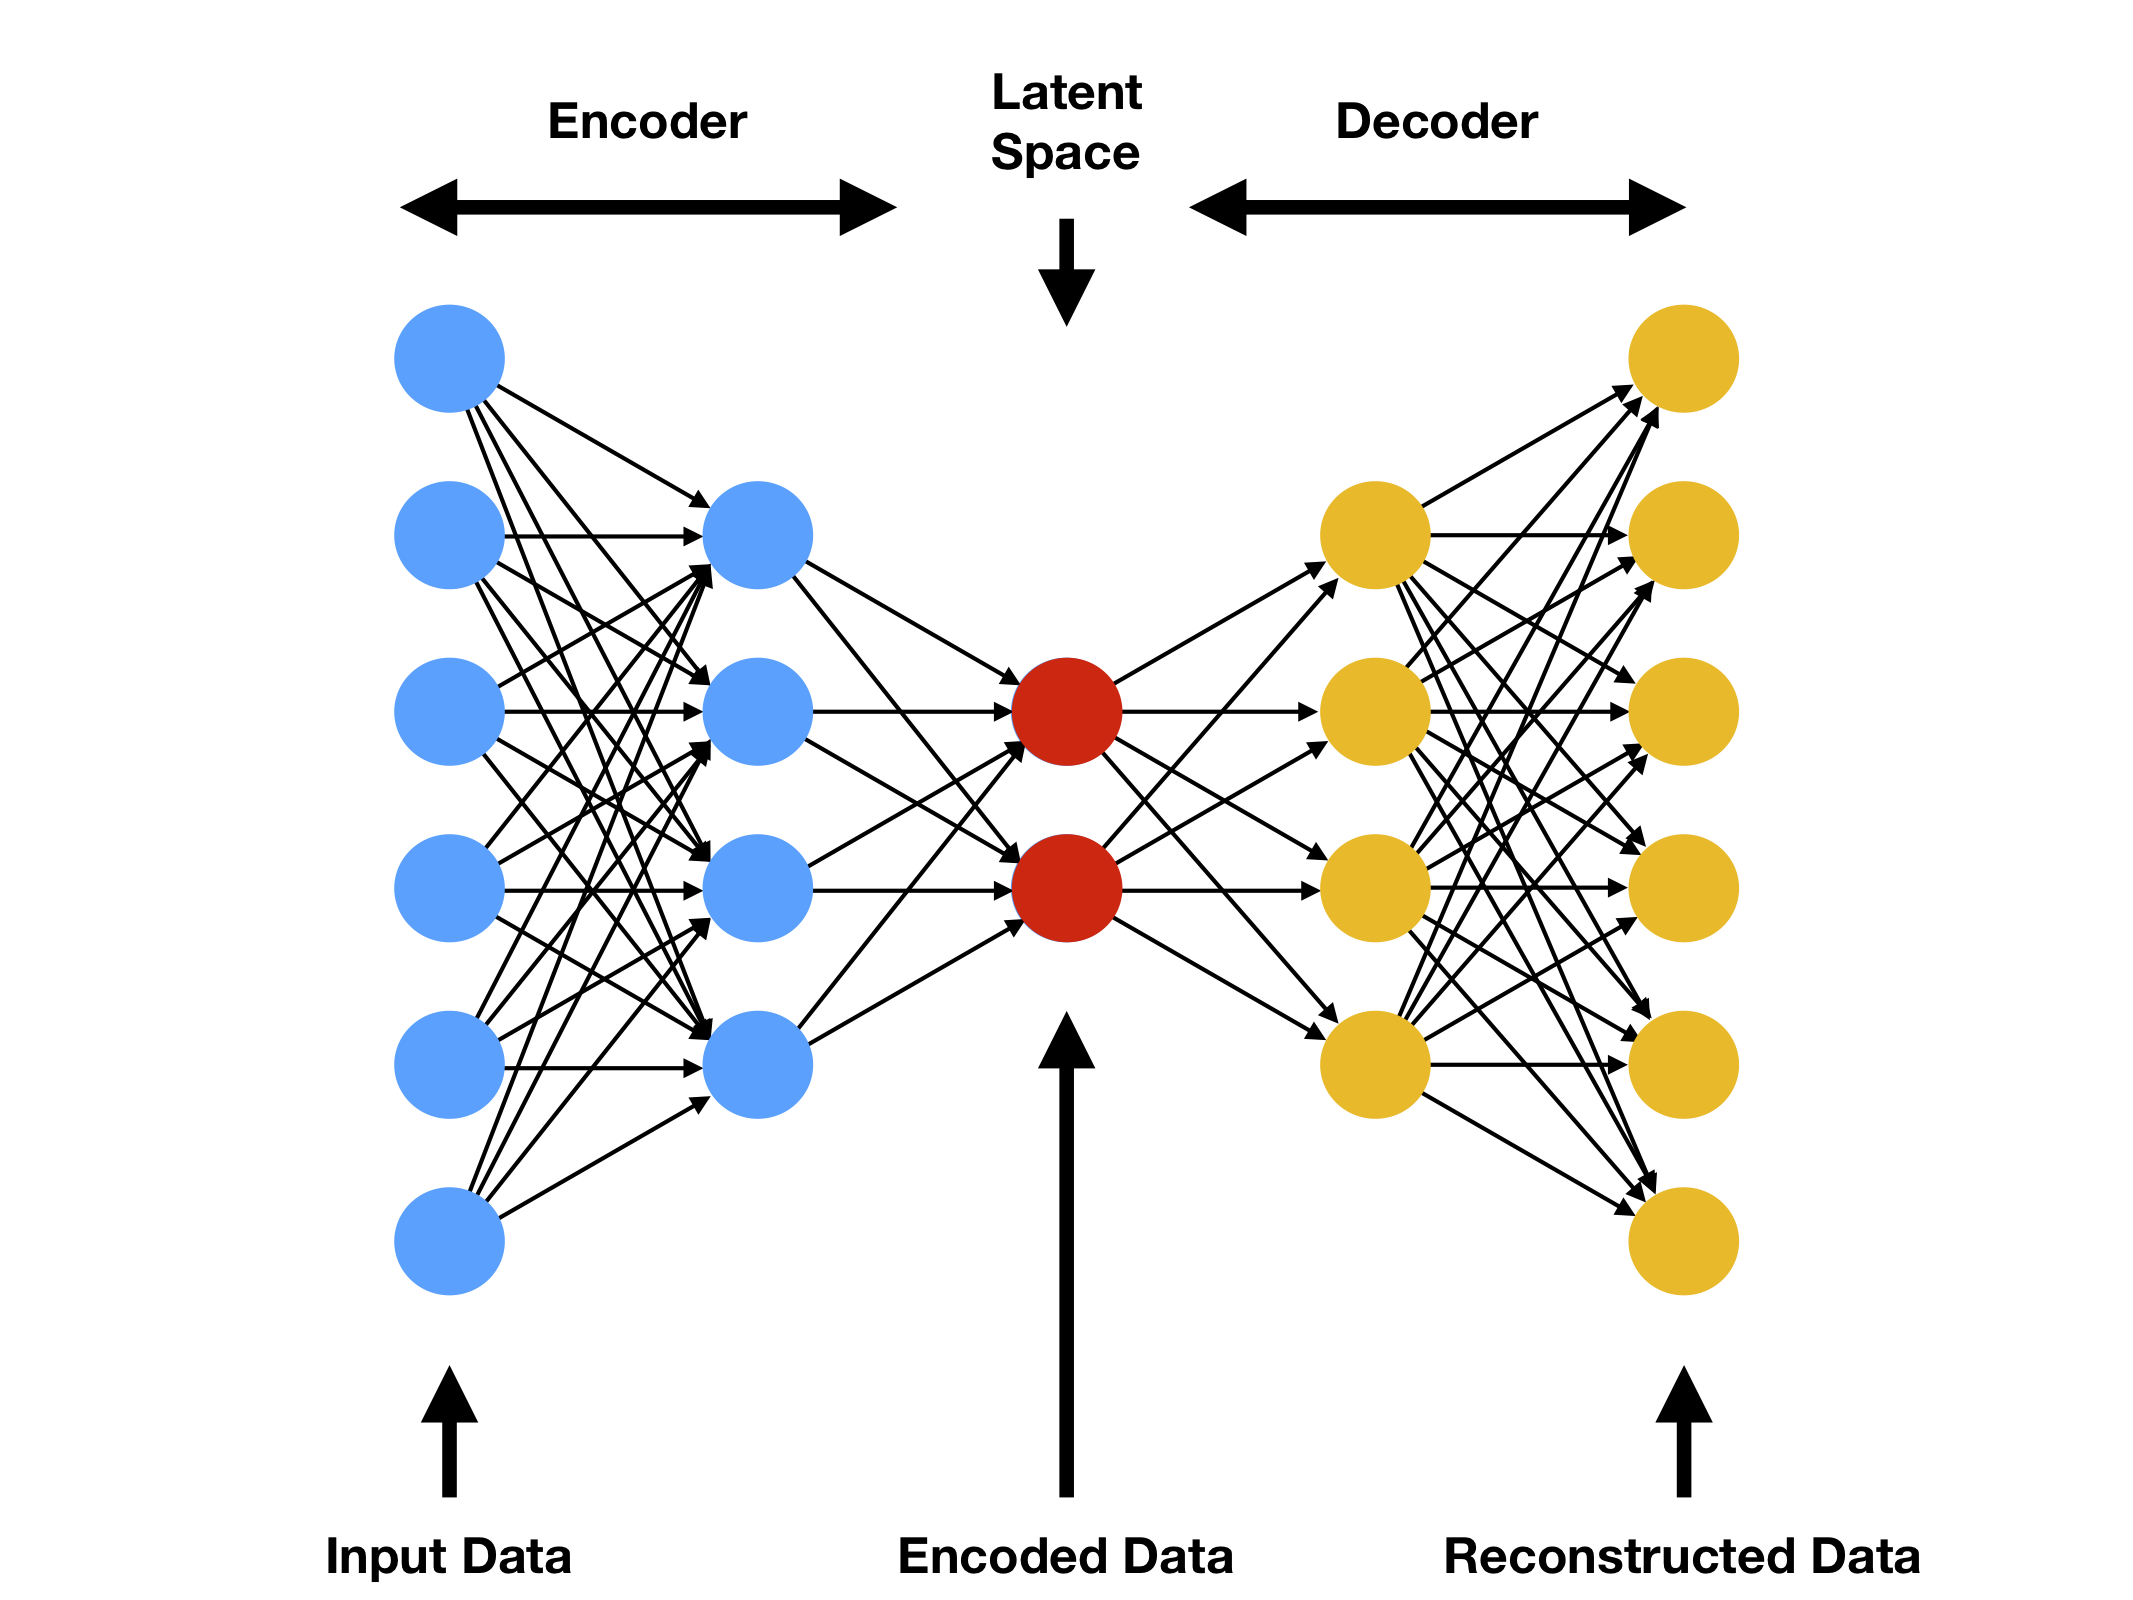
\includegraphics[width=\linewidth]{ae_5_layer.png}
    \caption{5 Layer Autoencoder}
    \label{fig:ae_5_layer}
\end{figure}

There is no established standard for autoencoder architecture for classification or anomaly detection problems. We use the architecture (16-8-4-2-4-8-16) in [4] as a baseline for performance comparison to measure the new architectures against. Table I summarizes the performance characteristics obtained by testing the baseline model. <TODO: add more explanation on Table 1> As shown in Figure 2, changing the number of nodes in layer 1 and layer 7 provides the performance impact to the F1 <TODO: additional sensitivity graphs, see email>score. As a performance metric for autoencoders and possibly all neural networks, complexity is the number of trainable parameters a network has. Reducing this number as much as possible is one of the goals of network architecture design.

\begin{table}
    \caption{BASELINE PERFORMANCE}
    \label{tab:baseline_metrics}
    \begin{center}
        \begin{tabular}{ |c|c| }
            \hline
            Performance metrics & Measured performance \\
            \hline
            F1 Score & 0.3287 \\
            \hline
            Recall & 0.6991 \\
            \hline
            Precision & 0.2148 \\
            \hline
            Accuracy & 0.4332 \\
            \hline
            Loss & 0.0095 \\
            \hline
            Complexity & 2,221 \\
            \hline

        \end{tabular}
    \end{center}
\end{table}

Precision is a relevance-based metric based on a percentage of correctly predicted or classified instances, and recall is the percentage of retrieved instances. One could simply classify all instances as one category and have 100\% recall, but with 0\% precision. A problem-specific balance between the two is optimal for best performance. F1 score is the harmonic mean between precision and recall and is used as the primary performance metric in both datasets. The F1 score has adjustable weights for how important precision is versus recall. To keep things simple and maintain the F1 score meaning between datasets, precision and recall are equally weighted in the calculation of F1 score for all results.

\begin{figure}
    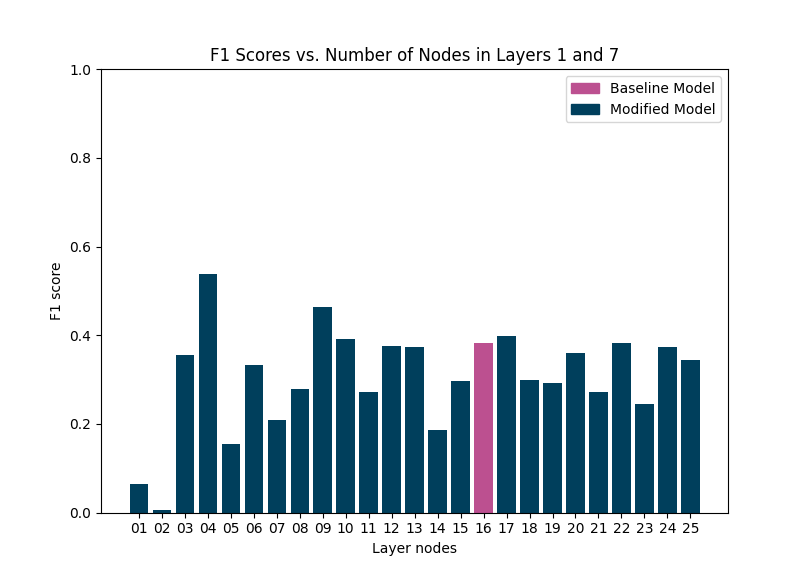
\includegraphics[width=\linewidth]{sensitivity_baseline_fraud_1.png}
    \caption{Sensitivity analysis of autoencoder architecture on credit card fraud dataset}
    \label{fig:sensitivity_fraud_1}
\end{figure}

\begin{figure}
    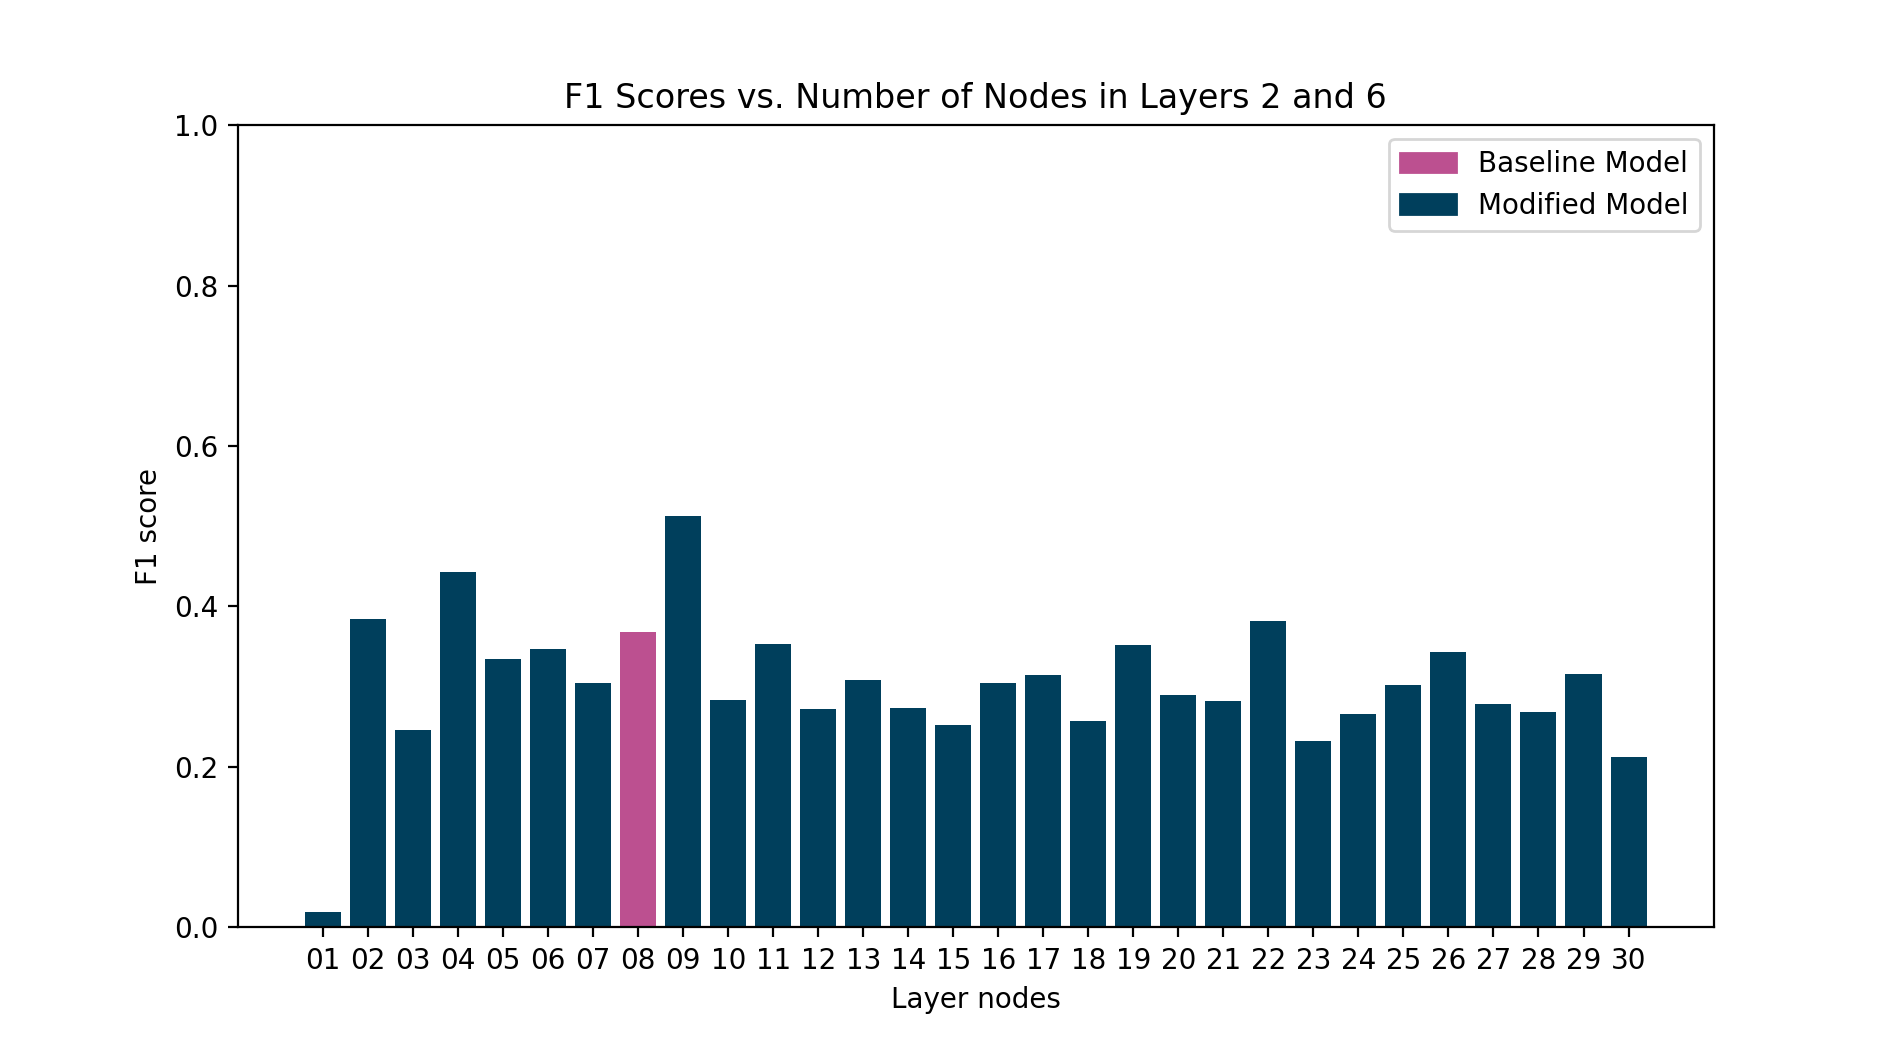
\includegraphics[width=\linewidth]{sensitivitiy_baseline_fraud_2.png}
    \caption{Sensitivity analysis of autoencoder architecture on credit card fraud dataset}
    \label{fig:sensitivity_fraud_2}
\end{figure}

\begin{figure}
    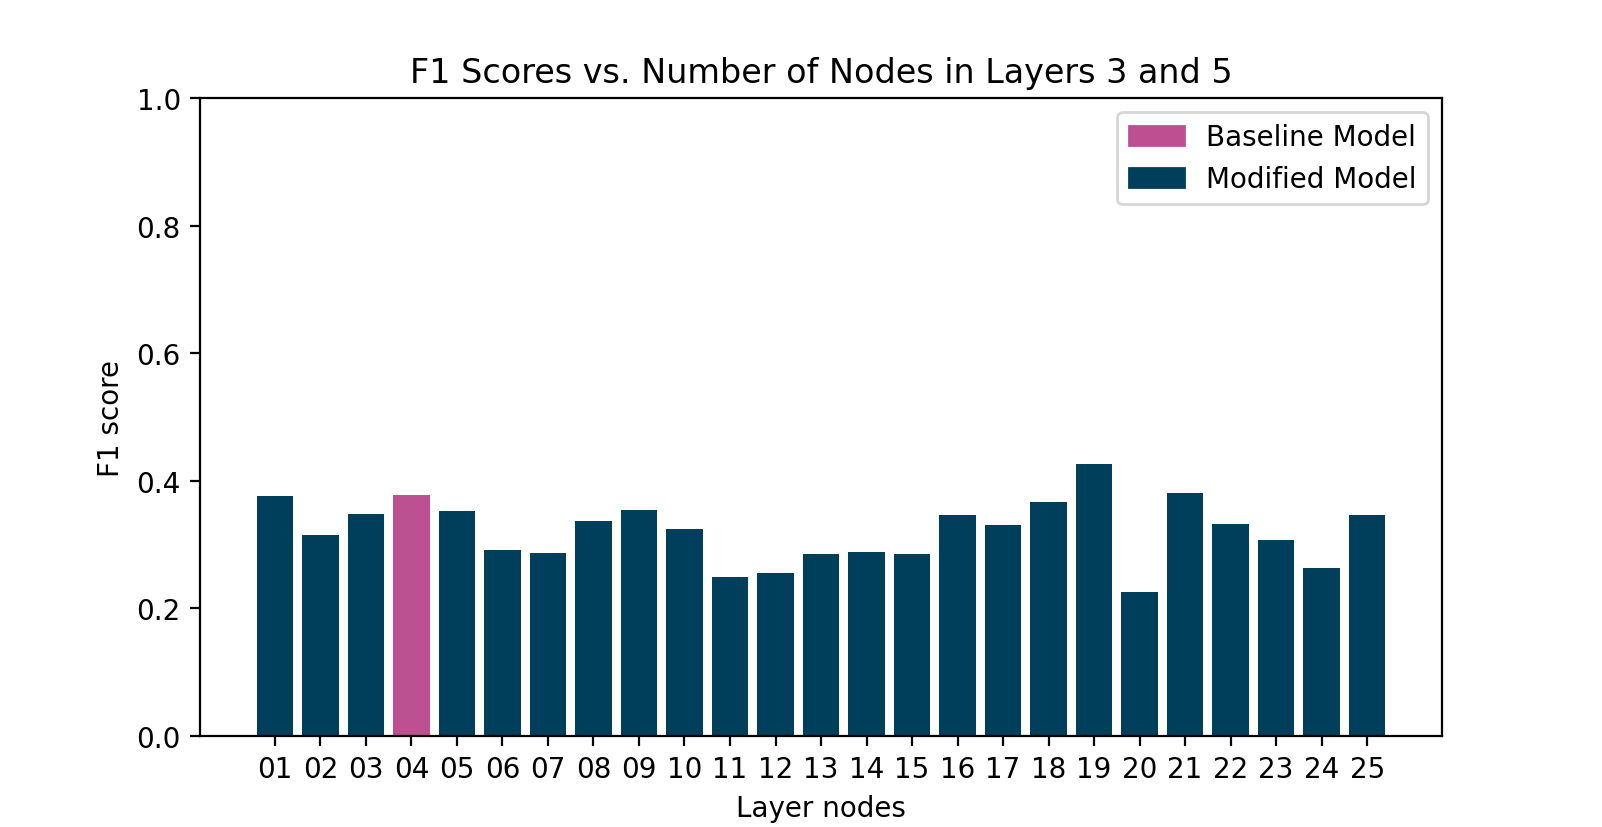
\includegraphics[width=\linewidth]{sensitivity_baseline_fraud_3.png}
    \caption{Sensitivity analysis of autoencoder architecture on credit card fraud dataset}
    \label{fig:sensitivity_fraud_3}
\end{figure}

%TODO: write about the figures above.

In figure \ref{fig:sensitivity_fraud_1} above, increasing and decreasing the number of nodes in layers 1 and 7 was tested. These sensitivity analysis results showed notable improvement in the decreasing of nodes rather than increasing which was unexpected as larger networks tend to perform better.

\section{Accordion AE ($A^2E$)}
When testing different potential autoencoder network architectures, one design generally worked better. Using the same number of layers as the baseline model introduced above in figure 2, the number of nodes in layers 2 and 6 were reduced to the number of nodes in the latent space. In this case, the layers containing 8 nodes were reduced to 2 nodes. This creates 3 layers where data being fed through is constrained to only 2 nodes essentially creating 3 individual latent spaces. In this new network, the number of nodes expand and contract creating a similar structure to that of multiple autoencoders connected together with the output of one connected to the input of the next. We decided to call this the accordion autoencoder.

The general concept of the accordion autoencoder is that data gets compressed and decompressed multiple times encouraging more meaningful features to be recorded at each compression stage. Essentially, it is an extension of the ability of the classic autoencoder to record meaningful features due to the memory capacity in the expansion layers immediately following each latent space layer. Presumably, the most mean- ingful features will end up in the last latent space after being ‘autoencoded’ several times to ensure only features which affect the reconstruction loss are present.
<TODO:
-All flat architecture (6-6-6-6-6) or (6-6-2-6-6)
-Accordion
-baseline
>

\section{Experiments and Analysis}

\subsection{Applications, dataset and performance metrics}
The applications for autoencoders explored in this paper involve anomaly detection which translates to detecting fraudulent credit card transactions and recognizing handwritten digits which is a classic image classification problem. The datasets are “Credit Card Fraud Detection” from Kaggle and “mnist” version 3.0.1 from Tensorflow respectively.

\begin{table}
    \caption{Characteristics of credit card fraud dataset}
    \label{tab:fraud_characteristics}
    \begin{center}
        \begin{tabular}{ |c|c| }
            \hline
            Total transactions & 84,807 \\
            \hline
            Total fraud transactions & 492 \\
            \hline
            Number of features & 29 \\
            \hline
        \end{tabular}
    \end{center}
\end{table}

\begin{table}
    \caption{Characteristics of MNIST dataset}
    \label{tab:mnist_characteristics}
    \begin{center}
        \begin{tabular}{ |c|c| }
            \hline
            Test images & 10,000 \\
            \hline
            Train images & 60,000 \\
            \hline
            Number of features & 784 \\
            \hline
        \end{tabular}
    \end{center}
\end{table}

Performance metrics measured in this analysis include:
\begin{itemize}
    \item Complexity
    \item Precision
    \item Recall
    \item Accuracy
    \item Loss
    \item F1 Score
\end{itemize}

\subsection{Methods}
\subsubsection{Credit Card Dataset}
Models were trained to reconstruct the 29 features of only the clean dataset. For privacy purposes, the dataset had already been modified using PCA \cite{kaggle_dataset} which results in 29 unlabeled fields. For testing, the mean absolute deviation (MAD) score was used to classify either fraud or clean data \cite{mad}. Since the model was only trained on clean data, it should have trouble reconstructing the fraud data resulting in a noticeably higher loss which is then used for classification. This is an unsupervised approach.
\subsubsection{MNIST Dataset}
For models used in MNIST image classification, a standard approach was used. The output layer of the model was always fixed at 10 nodes; one for each classification category. A combination of softmax activations and argmax was used to determine the classification categories in the predictions.

\subsection{Accuracy comparison: AE vs. $A^2E$}

\subsection{Network size comparison: AE vs. $A^2E$}

\subsection{Implications}

\section{Conclusion}

\section*{Acknowledgment}

\begin{thebibliography}{00}
    \bibitem{what_are_ae}https://arxiv.org/abs/2003.05991
    \bibitem{hinton_pca}https://www.cs.toronto.edu/~hinton/science.pdf
    \bibitem{complexity}http://math.bu.edu/people/mkon/nn30.pdf
    \bibitem{kaggle}https://www.kaggle.com/robinteuwens/anomaly-detection-with-auto-encoders
    \bibitem{kaggle_dataset}https://www.kaggle.com/mlg-ulb/creditcardfraud
    \bibitem{quantum}https://arxiv.org/pdf/1612.02806.pdf
    \bibitem{mad}https://arxiv.org/abs/1901.04997
\end{thebibliography}

\vspace{12pt}
\color{red}

\end{document}
